\chapter{Stromal and Oncogenic Regulation of Colonic Stem Cell Polarisation}
\label{04seq}

\section{Introduction}


AIMS
% Both the SI LGR5 and the colonic organoid systems have been thoroughly characterised before at the mass cytometry level and, to better understand these systems, we aim to perform a comparative characterisation of the organoids using scRNA-seq. 
% Given the well-known biology of the murine small intestine at the transcriptome level21, we can analyse the SI LGR5s to characterise the different subpopulations within the epithelial organoids and cross-validate the results with in vivo scRNA-seq studies and the mass cytometry results discussed above11. In a similar fashion, we also aim to characterise the colonic organoids and the stromal and immune compartments that form the TME in the heterocellular cultures. Unlike mass cytometry, which requires tailored panels of antibodies reaching only into a few dozens, with scRNA-seq we will be able to characterise thousands of genes at once in the organoids, fibroblasts, and macrophages. 
% Leveraging the publicly available ligand-receptor databases mentioned in the background section, data from the scRNA-seq experiments will be used to identify the ligands and receptors expressed in the colonic heterocellular organoid cocultures. 
% The cell communication information gathered this way can then be summarised as signalling pathways that define and connect the different populations of cells. Furthermore, the study of this interactome would aid towards understanding the interplay between the CRC organoid model and its TME. This can be achieved by comparing the cell communication results with the intracellular PTM signalling described in Qin et al. 2020 and seeing how cellular communications change in cultures mimicking an oncogenic setting.

\subsubsection{Figure on experimental design, with the 2 axes of perturbation}

\begin{figure}
    \centering
    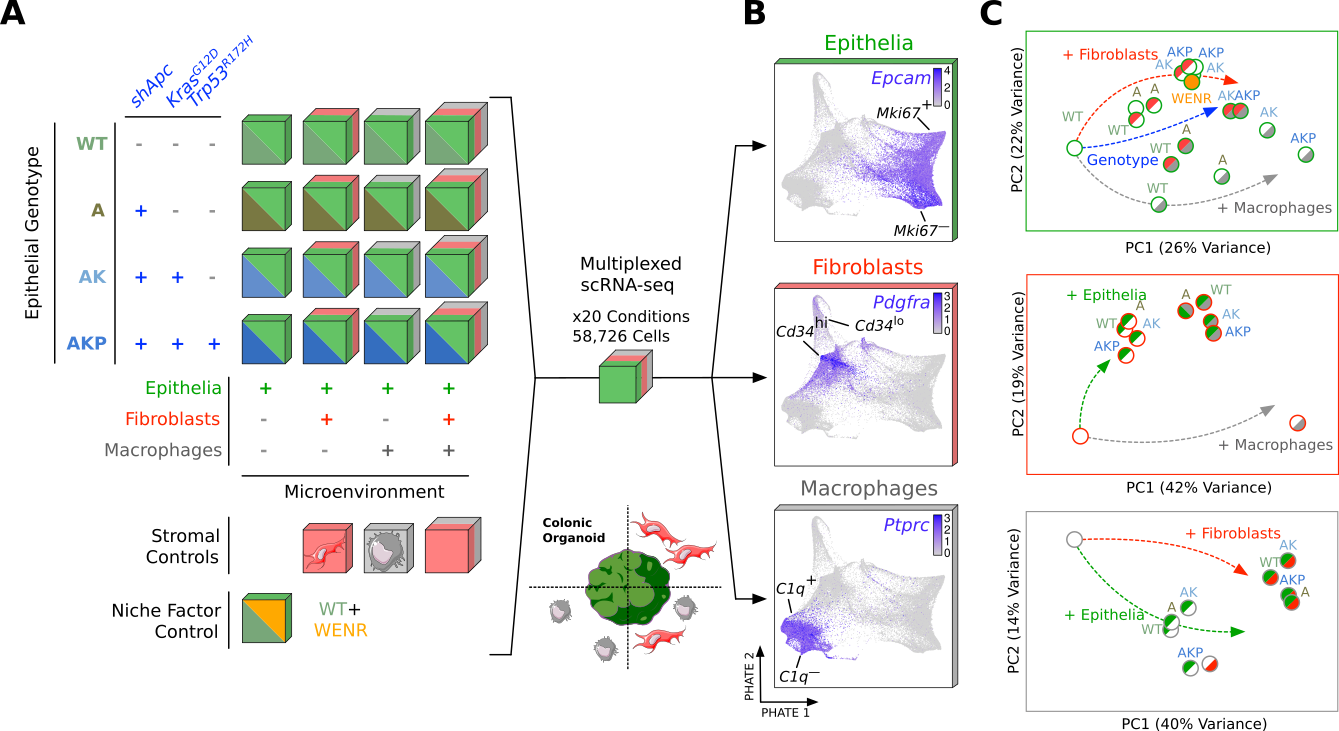
\includegraphics{04seq/figs/4SEQ_ExpDesign.png}
    \caption{}
    \label{fig:}
\end{figure}

\section{Organoids recapitulate colonic epithelial cell states}

\subsubsection{Figure on Integrated object DR, and expression of cannonical markers in control condition}
\begin{figure}
    \centering
    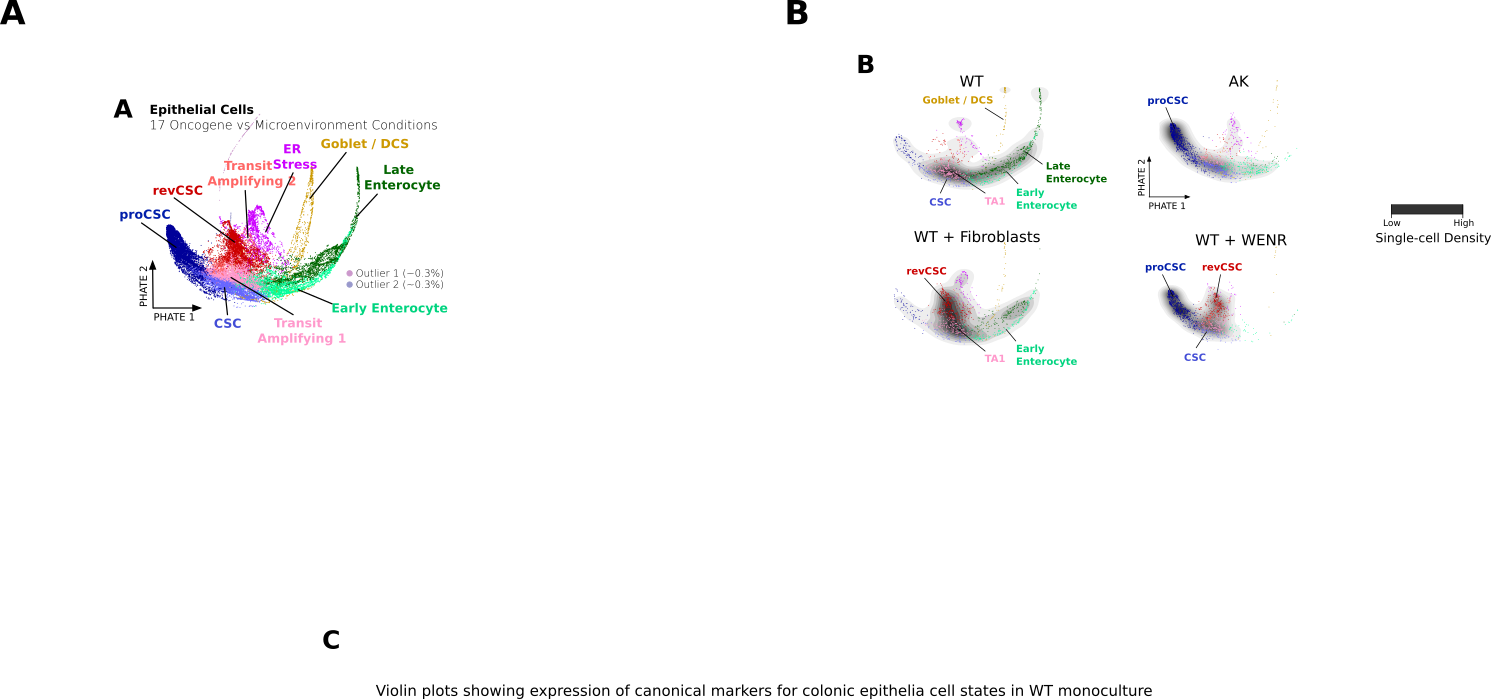
\includegraphics{04seq/figs/4SEQ_INTctrl.png}
    \caption{}
    \label{fig:}
\end{figure}

\section{Oncogenic mutations and fibroblasts polarise epithelia towards distinct stem cell fates}

\subsubsection{Figure on DA overview and individual DA tests}

\begin{figure}
    \centering
    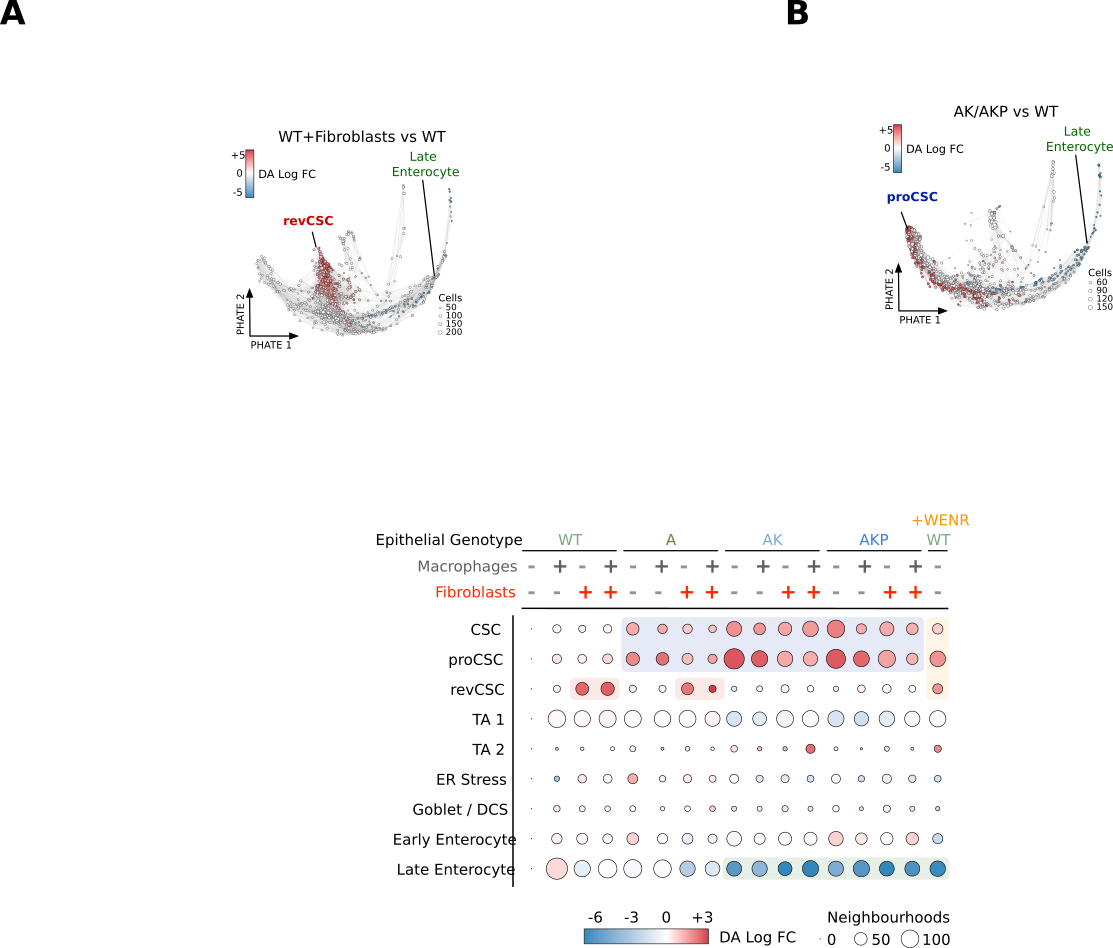
\includegraphics{04seq/figs/4SEQ_DA.png}
    \caption{}
    \label{fig:}
\end{figure}

\begin{figure}
    \centering
    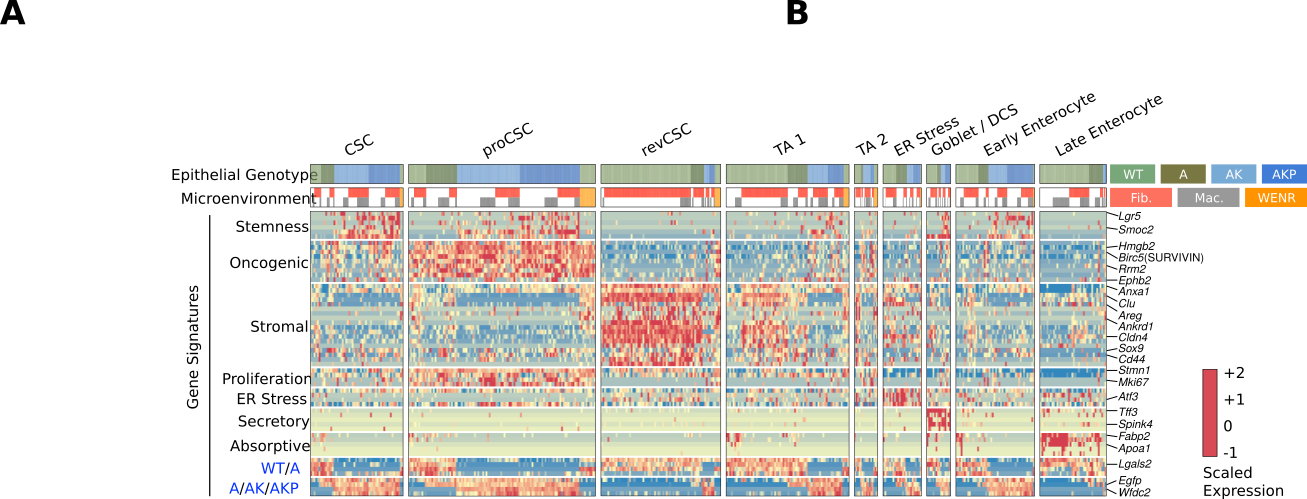
\includegraphics{04seq/figs/4SEQ_DE.png}
    \caption{}
    \label{fig:}
\end{figure}

\subsubsection{Figure on signalling entropy, RNA velocity changes, and CellRank sinks}

\begin{figure}
    \centering
    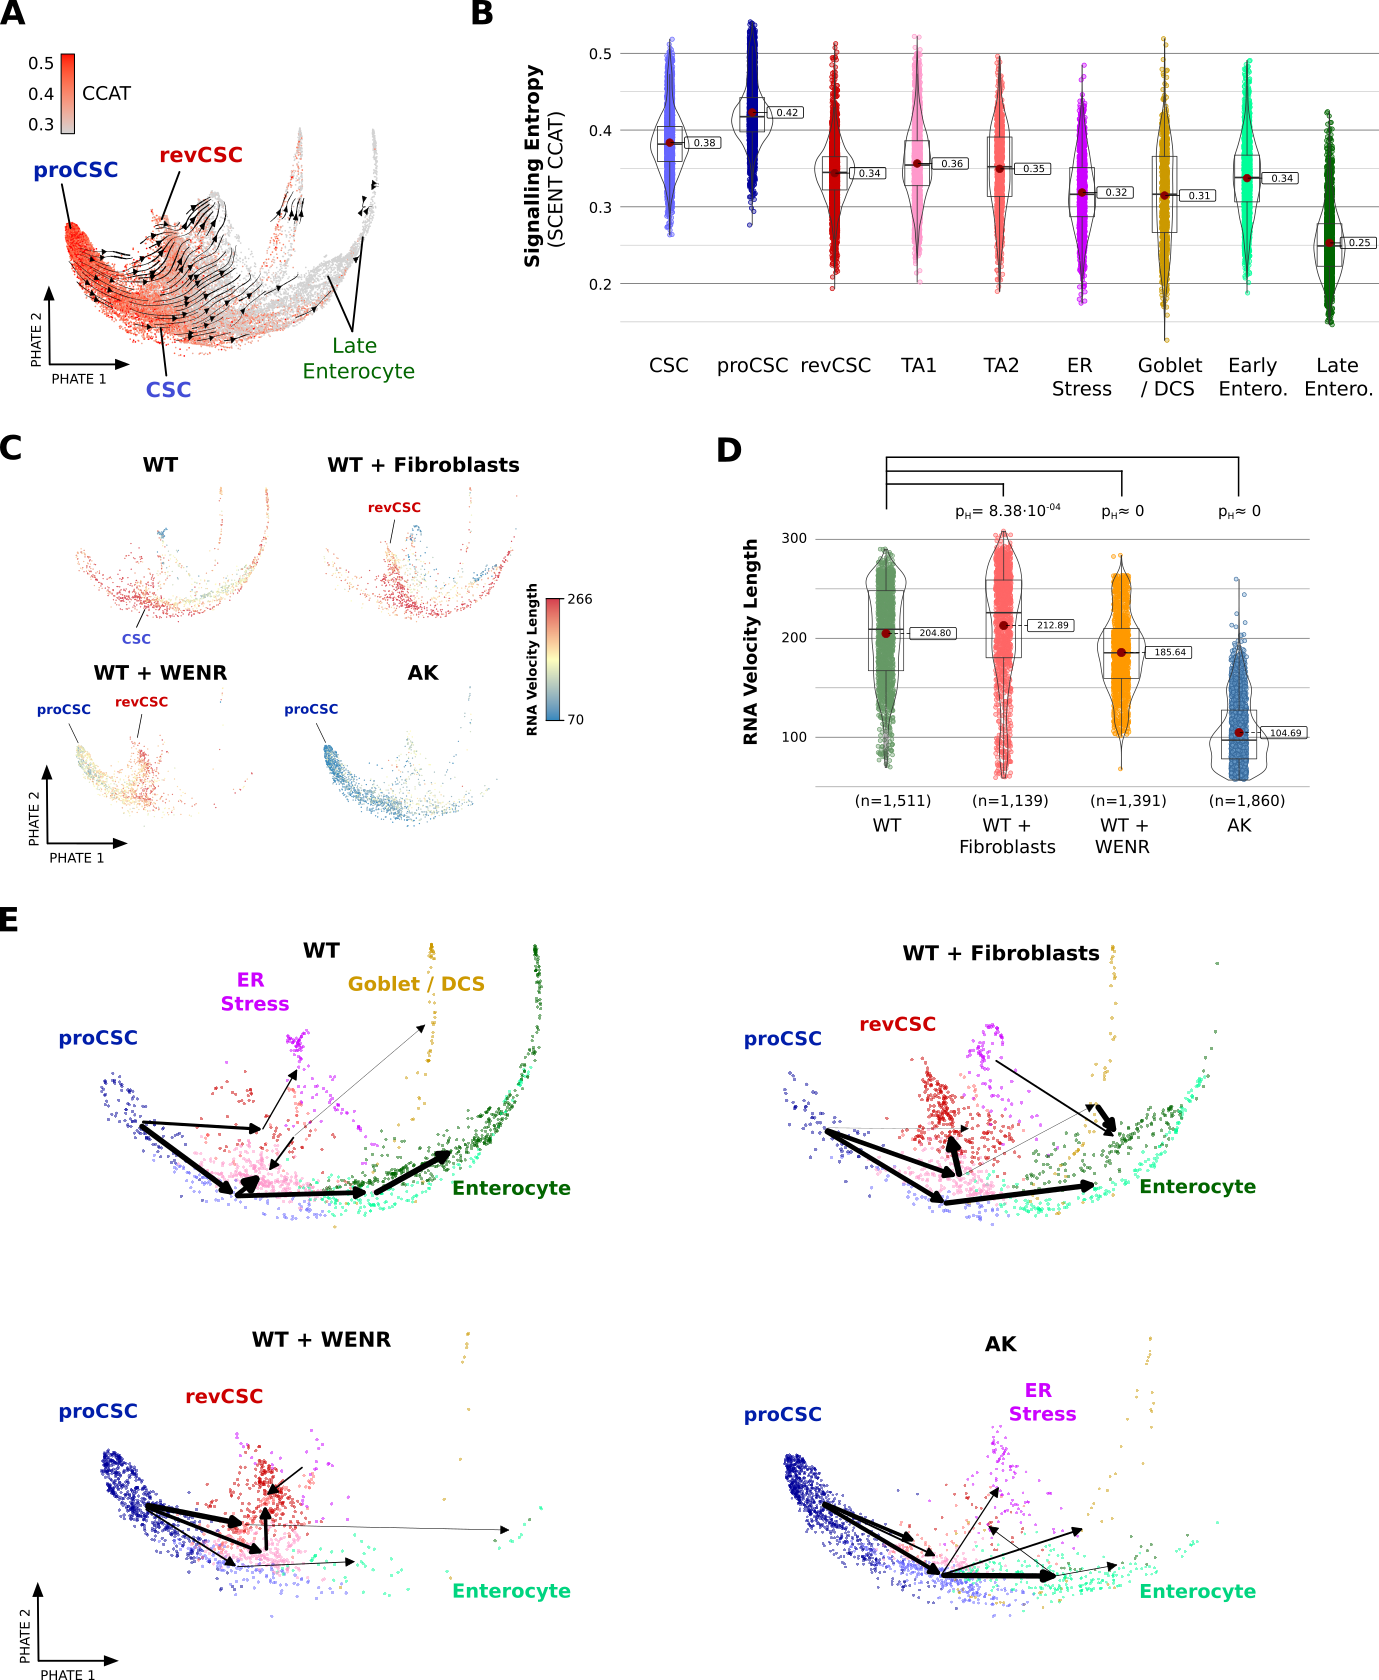
\includegraphics{04seq/figs/4SEQ_Dynamics.png}
    \caption{}
    \label{fig:}
\end{figure}

\section{Oncogenic mutations block fibroblast to epithelia signalling}

\subsubsection{Figure on cell-cell communication analysis}

\begin{figure}
    \centering
    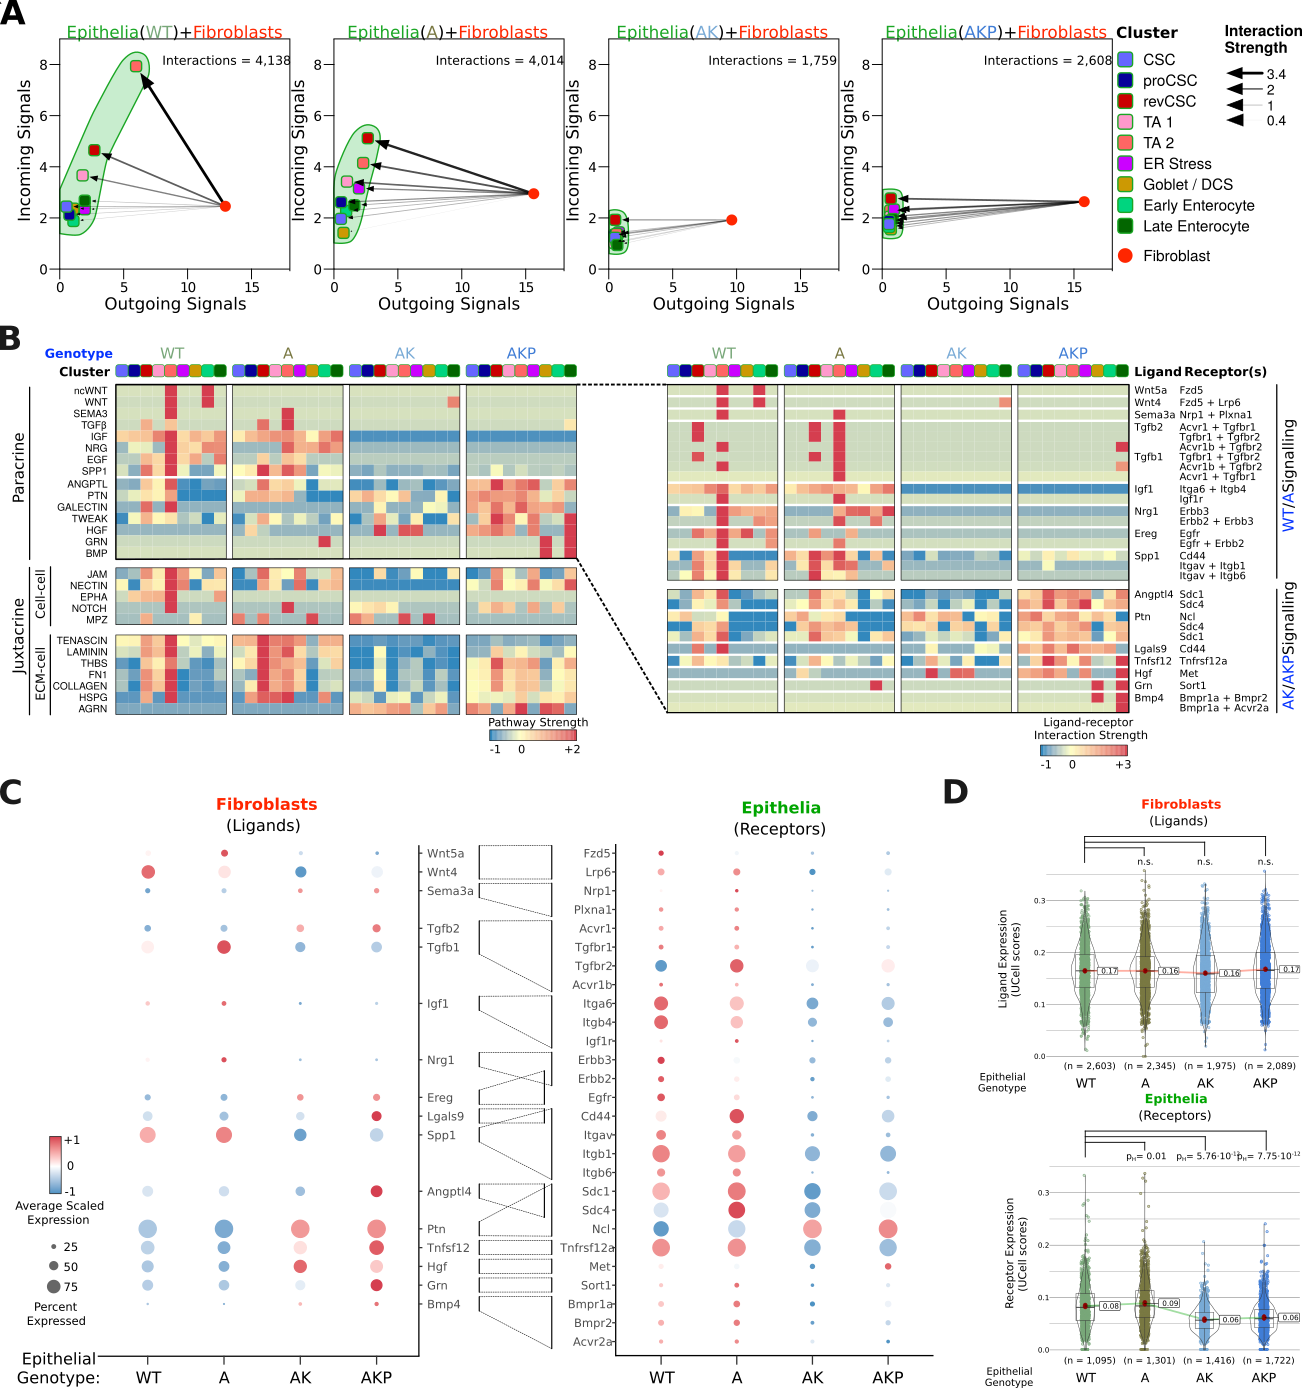
\includegraphics{04seq/figs/4SEQ_CC.png}
    \caption{}
    \label{fig:}
\end{figure}

\section{Characterisation and relevance of proCSC and revCSC}

\subsubsection{Figure on stem signatures and key signalling pathways}

\begin{figure}
    \centering
    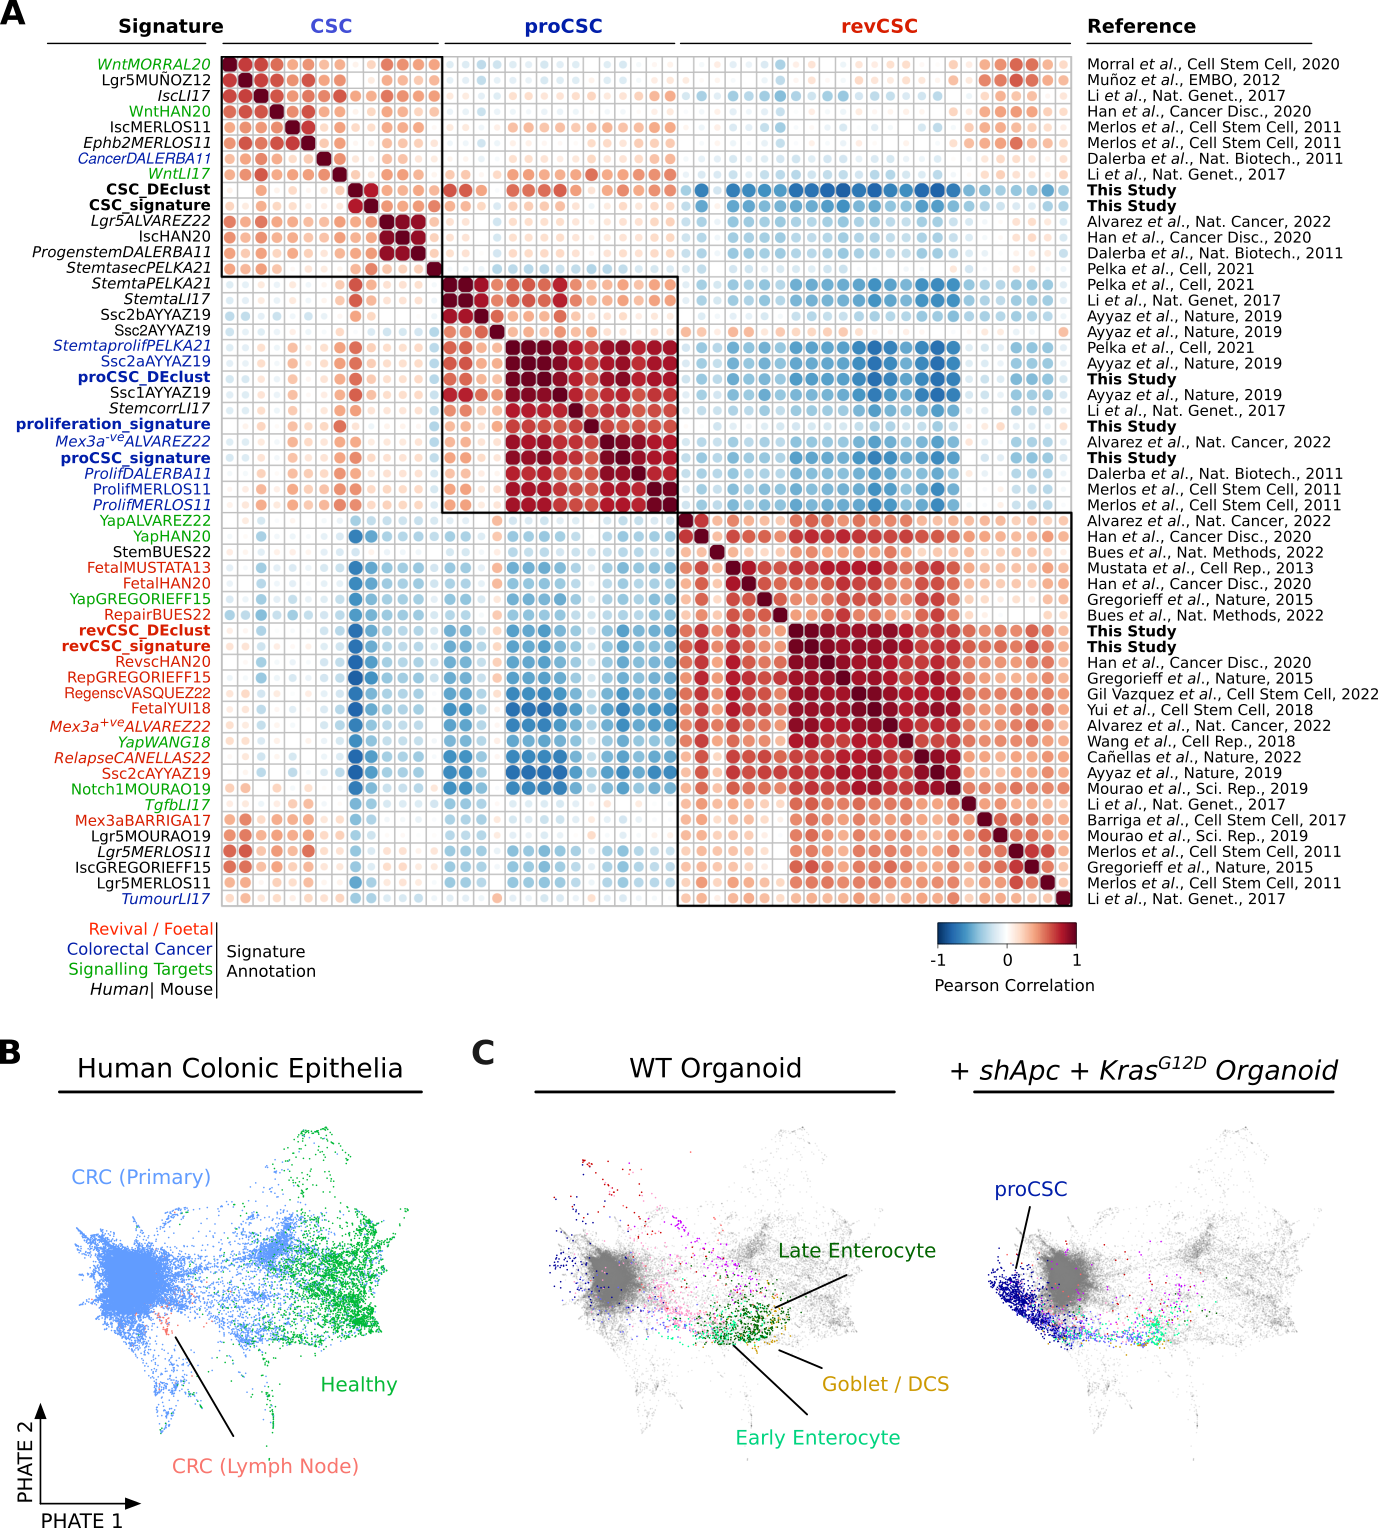
\includegraphics{04seq/figs/4SEQ_StemSign.png}
    \caption{}
    \label{fig:}
\end{figure}

\section{Conclusions}





